\documentclass[11pt]{article}

\usepackage[margin=1in]{geometry}
\usepackage[T1]{fontenc}
\usepackage{lmodern}
\usepackage{microtype}
\usepackage{amsmath,amssymb,amsthm,mathtools}
\usepackage{mathrsfs}
\usepackage[dvipsnames]{xcolor}
\usepackage[most]{tcolorbox}
\usepackage{tikz}
\usetikzlibrary{decorations.markings,patterns}
\usepackage{enumitem}
\usepackage{tocloft}
\usepackage[hidelinks]{hyperref}

\definecolor{courseblue}{HTML}{1F4E79}
\definecolor{lightblue}{HTML}{EAF2F8}
\definecolor{lightgreen}{HTML}{EAF7EA}
\definecolor{lightpink}{HTML}{FCE8EF}
\definecolor{lightyellow}{HTML}{FFF8D6}
\definecolor{warningyellow}{HTML}{D6A000}
\definecolor{exercisebg}{HTML}{FDEAEA}
\definecolor{exerciseframe}{HTML}{B54040}
\definecolor{examplebg}{HTML}{F4FAFE}
\definecolor{exampleframe}{HTML}{85C1E9}
\definecolor{darkgray}{HTML}{333333}
\definecolor{lightorange}{HTML}{FDEBD8}
\definecolor{orangeframe}{HTML}{E08A3C}
\definecolor{remarkbg}{HTML}{F3EEFB}
\definecolor{remarkframe}{HTML}{9B7FC9}

\setlength{\parindent}{0pt}
\setlength{\parskip}{0.45em}
\setlist[itemize]{topsep=0.25em,itemsep=0.15em}
\renewcommand{\cftsecleader}{\cftdotfill{\cftdotsep}}
\renewcommand{\cftsubsecleader}{\cftdotfill{\cftdotsep}}

\theoremstyle{plain}
\newtheorem{theorem}{Theorem}[section]
\newtheorem{proposition}[theorem]{Proposition}
\newtheorem{lemma}[theorem]{Lemma}
\newtheorem{corollary}[theorem]{Corollary}
\theoremstyle{definition}
\newtheorem{definition}[theorem]{Definition}
\newtheorem{example}[theorem]{Example}
\newtheorem{exercise}[theorem]{Exercise}
\theoremstyle{remark}
\newtheorem*{remark}{Remark}
\newtheorem*{fact}{Fact}
\newtheorem*{warning}{Warning}

\tcolorboxenvironment{definition}{
  enhanced,
  unbreakable,
  colback=lightgreen,
  colframe=ForestGreen,
  boxrule=0.7pt,
  arc=2pt,
  left=6pt,
  right=6pt,
  top=5pt,
  bottom=5pt
}

\tcolorboxenvironment{remark}{
  enhanced,
  colback=remarkbg,
  colframe=remarkframe,
  before upper={\setlength{\parskip}{0.5em}},
  boxrule=0.7pt,
  arc=2pt,
  left=6pt,
  right=6pt,
  top=5pt,
  bottom=5pt
}

\tcolorboxenvironment{warning}{
  enhanced,
  colback=lightyellow,
  colframe=warningyellow,
  boxrule=0.7pt,
  arc=2pt,
  left=6pt,
  right=6pt,
  top=5pt,
  bottom=5pt
}

\tcolorboxenvironment{exercise}{
  enhanced,
  colback=exercisebg,
  colframe=exerciseframe,
  boxrule=1pt,
  arc=2pt,
  left=6pt,
  right=6pt,
  top=5pt,
  bottom=5pt
}

\tcolorboxenvironment{example}{
  enhanced,
  colback=examplebg,
  colframe=exampleframe,
  boxrule=0.7pt,
  arc=2pt,
  left=6pt,
  right=6pt,
  top=5pt,
  bottom=5pt
}

\numberwithin{equation}{section}

\newcommand{\be}{\begin{eqnarray}}
\newcommand{\ee}{\end{eqnarray}}
\newcommand{\C}{\mathbb{C}}
\newcommand{\R}{\mathbb{R}}
\newcommand{\N}{\mathbb{N}}
\newcommand{\Z}{\mathbb{Z}}
\DeclareMathOperator{\Log}{Log}
\DeclareMathOperator{\Arg}{Arg}

\DeclareMathOperator{\Hol}{\mathcal{H}\mathrm{ol}}
\DeclareMathOperator{\Real}{Re}
\DeclareMathOperator{\Imag}{Im}
\newcommand{\A}{\mathcal{A}}
\newcommand{\CT}{\C[[T]]}
\newcommand{\CLT}{\C((T))}
\tcbset{breakable}
% Compact spacing around diagrams; keep the main text at 11pt.
\newenvironment{lecturefigure}
 {\par\addvspace{0.25em}\begingroup\setlength{\parskip}{0pt}\centering}
 {\par\endgroup\addvspace{0.25em}}
\begin{document}

\begin{center}
  \colorbox{lightblue}{%
    \begin{minipage}{0.94\textwidth}
      \vspace{0.55em}
      \begin{tabular*}{\textwidth}{@{\extracolsep{\fill}}lr}
        {\color{courseblue}\bfseries\LARGE Lecture 24} &
        {\color{courseblue}\bfseries\LARGE MATH 411}\\[0.35em]
        \textbf{Fall 2026} & \textbf{Date: Nov 4, 2026}\\
        & \textbf{Instructor: Manish Patnaik}
      \end{tabular*}
      \vspace{0.45em}
    \end{minipage}}
\end{center}

\setcounter{tocdepth}{1}
\tableofcontents
\vspace{0.45em}

% Sources: handwritten Lecture 24, Nov. 14, pages 1--6. Order follows the
% handwritten notes: recall of the residue theorem, order of a zero or
% pole via the logarithmic derivative, the argument principle, Rouche's
% theorem with an application and proof, the open mapping theorem.
% Added: a lemma on zeros of holomorphic functions (needed for finiteness
% of zeros in Rouche's theorem and for the open mapping theorem), an
% explicit continuity estimate in the proof of Rouche, and the
% connectedness hypothesis in the open mapping theorem.
Last time we proved the residue theorem and used it to compute integrals.
Today we give \emph{theoretical} applications: counting zeros and poles
with the argument principle, comparing zeros of two functions with
Rouch\'e's theorem, and proving that nonconstant holomorphic functions are
open maps.

\section{Meromorphic functions and the order of a zero or pole}
% Handwritten Lecture 24, pages 1--2.
\subsection{Recall: the residue theorem}
A function $f$ is \emph{meromorphic} on an open set $U$ if it is
holomorphic on $U$ except for poles. In Lecture~23 we proved: if $f$ is
holomorphic on $U$ except at $z_1,\dots,z_n$, and $\gamma$ is a closed
curve in $U\setminus\{z_1,\dots,z_n\}$ that is null-homotopic in $U$, then
\[
 \int_\gamma f=2\pi i\sum_{j=1}^{n}
 \underbrace{w(\gamma,z_j)}_{\text{winding number}}\,
 \underbrace{\operatorname{Res}_{z_j}(f)}_{\text{residue of $f$ at $z_j$}}.
\]

\subsection{Zeros of holomorphic functions}
We need a fact about zeros which we have so far only proved for power
series (Lecture~10).

\begin{lemma}[Zeros are isolated]\label{lem:zeros}
Let $D$ be a connected open set and $F$ holomorphic on $D$, not
identically zero. Then:
\begin{enumerate}
 \item at each zero $z_0$ of $F$ there are an integer $m\geq1$ and a
 function $g$ holomorphic near $z_0$ with $g(z_0)\ne0$ such that
 $F(z)=(z-z_0)^mg(z)$; in particular $z_0$ is an isolated zero;
 \item $F$ has only finitely many zeros in each compact subset of $D$.
\end{enumerate}
\end{lemma}
\begin{proof}
Let $S=\{z\in D:\ F^{(k)}(z)=0\text{ for all }k\geq0\}$. Each derivative
is continuous, so $S$ is closed in $D$. If $z\in S$, the Taylor series of
$F$ at $z$ is zero, and it represents $F$ on a disc around $z$
(Lecture~20); so $F\equiv0$ on that disc, which therefore lies in $S$.
Thus $S$ is also open. Since $D$ is connected and $S\ne D$, we get
$S=\emptyset$.

(1) At a zero $z_0$, let $m\geq1$ be the least $k$ with
$F^{(k)}(z_0)\ne0$. The Taylor series at $z_0$ starts with
$a_m(z-z_0)^m$, $a_m\ne0$, so $F=(z-z_0)^mg$ with
$g(z)=a_m+a_{m+1}(z-z_0)+\cdots$. Since $g(z_0)\ne0$ and $g$ is
continuous, $g$ and hence $F$ has no other zeros near $z_0$.

(2) If $K\subseteq D$ is compact and contains infinitely many zeros, they
accumulate at some $p\in K$. By continuity $F(p)=0$, and $p$ is not an
isolated zero, contradicting (1).
\end{proof}

\subsection{Order and the logarithmic derivative}
Let $f$ be meromorphic near $z_0$ and not identically zero near $z_0$. By
Lemma~\ref{lem:zeros} if $f(z_0)=0$, and by the Laurent expansion
(Lecture~22) if $z_0$ is a pole, we can write
\[
 f(z)=(z-z_0)^m\,g(z),\qquad g\text{ holomorphic near }z_0,\quad g(z_0)\ne0,
\]
for a unique integer $m$. Equivalently, $f(z)=a_m(z-z_0)^m(1+h(z))$ with
$a_m=g(z_0)\ne0$ and $h$ holomorphic, $h(z_0)=0$.

\begin{definition}
The integer $m=\operatorname{ord}_{z_0}(f)$ is the \emph{order} of $f$
at $z_0$. If $m>0$, $f$ has a \emph{zero of order $m$}; if $m<0$, $f$ has a
\emph{pole of order $-m$}. For example, $m=-1$ means
$f=\frac{a_{-1}}{z-z_0}+\cdots$, a pole of order $1$.
\end{definition}

By the product rule $(fg)'=f'g+fg'$, so
\[
 \frac{(fg)'}{fg}=\frac{f'}{f}+\frac{g'}{g}.
\]
The quotient $f'/f$ is called the \emph{logarithmic derivative} of $f$,
written $d\log(f)$, since formally $(\log f)'=f'/f$. The identity says
$d\log(fg)=d\log(f)+d\log(g)$. Applying it to $f=(z-z_0)^m\cdot g$,
\[
 \frac{f'}{f}=\frac{m}{z-z_0}+\frac{g'}{g}.
\]
Since $g(z_0)\ne0$, $g'/g$ is holomorphic near $z_0$. Hence
\[
 \boxed{\operatorname{Res}_{z_0}\Bigl(\frac{f'}{f}\Bigr)
 =m=\operatorname{ord}_{z_0}(f).}
\]

\section{The argument principle}
% Handwritten Lecture 24, pages 2--3.
Combining this observation with the residue theorem:

\begin{theorem}\label{thm:log-derivative}
Let $U$ be open and $f$ meromorphic on $U$ with finitely many zeros and
poles $z_1,\dots,z_n$. Let $\gamma$ be a closed curve in
$U\setminus\{z_1,\dots,z_n\}$ that is null-homotopic in $U$. Then
\[
 \int_\gamma\frac{f'}{f}=2\pi i\sum_{j=1}^{n}w(\gamma,z_j)\,
 \operatorname{ord}_{z_j}(f).
\]
\end{theorem}
\begin{proof}
On $U\setminus\{z_1,\dots,z_n\}$, $f$ is holomorphic and nonvanishing, so
$f'/f$ is holomorphic there. At each $z_j$ it has residue
$\operatorname{ord}_{z_j}(f)$ by the computation above. Apply the residue
theorem to $f'/f$.
\end{proof}

\begin{example}
Let $f(z)=\dfrac{(z-1)^2}{(z+2)^3}$, with a zero of order $2$ at $1$ and a
pole of order $3$ at $-2$. For the circle $|z|=3$, both points are inside
and $\int f'/f=2\pi i(2-3)=-2\pi i$. For $|z|=\tfrac32$, only $1$ is inside
and $\int f'/f=4\pi i$. Directly,
$f'/f=\frac{2}{z-1}-\frac{3}{z+2}$.
\end{example}

Choosing $\gamma$ to be a circle gives the following.

\begin{corollary}[Argument principle]\label{cor:argument}
Let $C$ be a positively oriented circle bounding the open disc $D$, and
let $f$ be meromorphic on an open set $W\supseteq\overline D$, with finitely
many zeros and poles in $W$, none on $C$. Then
\[
 \boxed{\frac{1}{2\pi i}\int_C\frac{f'}{f}
 =\#\{\text{zeros of $f$ in $D$}\}-\#\{\text{poles of $f$ in $D$}\},}
\]
where zeros and poles are counted with multiplicity (that is, with their
orders).
\end{corollary}
\begin{proof}
Let $D=D(c,r)$. By compactness of $\overline D$ there is $\rho>r$ with
$D(c,\rho)\subseteq W$. Apply Theorem~\ref{thm:log-derivative} on the
convex, hence simply connected, set $U=D(c,\rho)$. It remains to note that
$w(C,\alpha)=1$ for $\alpha\in D$ (Cauchy's formula with $f=1$) and
$w(C,\alpha)=0$ for $|\alpha-c|>r$ (since $1/(z-\alpha)$ is holomorphic on
the disc $D(c,|\alpha-c|)$, which contains $C$).
\end{proof}

\begin{lecturefigure}
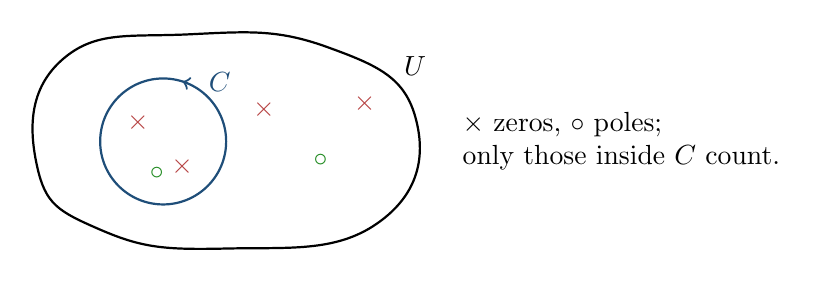
\begin{tikzpicture}[scale=0.8]
 \draw[thick] plot[smooth cycle,tension=0.8] coordinates
 {(-3,-0.4) (-2.6,1.3) (-0.6,1.7) (1.6,1.5) (3,0.4)
  (2.4,-1.3) (0,-1.7) (-2,-1.4)};
 \node at (3,1.2) {$U$};
 \draw[courseblue,thick,postaction={decorate},decoration={markings,
  mark=at position 0.2 with {\arrow{>}}}] (-1,0) circle(1);
 \node[courseblue] at (-0.1,0.95) {$C$};
 \node[exerciseframe] at (-1.4,0.3) {$\times$};
 \node[exerciseframe] at (-0.7,-0.4) {$\times$};
 \node[ForestGreen] at (-1.1,-0.5) {$\circ$};
 \node[exerciseframe] at (0.6,0.5) {$\times$};
 \node[ForestGreen] at (1.5,-0.3) {$\circ$};
 \node[exerciseframe] at (2.2,0.6) {$\times$};
 \node[right,align=left] at (3.6,0)
 {$\times$ zeros, $\circ$ poles;\\ only those inside $C$ count.};
\end{tikzpicture}
\end{lecturefigure}

\begin{remark}[Why ``argument'']
If $C$ is parametrized by $\gamma(t)$, $0\leq t\leq2\pi$, then
$\int_C f'/f=\int_0^{2\pi}\frac{(f\circ\gamma)'(t)}{f(\gamma(t))}\,dt
=\int_{f\circ C}\frac{dw}{w}$. So the left side of the argument principle
is $w(f\circ C,0)$: the number of times the image curve $f\circ C$ winds
around $0$, i.e.\ the total change in $\arg f(z)$ around $C$, divided by
$2\pi$.
\end{remark}

\section{Rouch\'e's theorem}
% Handwritten Lecture 24, pages 3--5.
\begin{theorem}[Rouch\'e's theorem]\label{thm:rouche}
Let $f$ and $g$ be holomorphic on an open set containing a closed disc
$\overline D$ with boundary circle $C$, and suppose
\[
 |f(z)|>|g(z)|\qquad\text{for all }z\in C.
\]
Then $f$ and $f+g$ have the same number of zeros in $D$, counted with
multiplicity.
\end{theorem}
Note that the hypothesis forces $f\ne0$ on $C$. Think of $g$ as a
perturbation that is small on $C$: it does not change the number of zeros
inside.

\begin{example}
How many zeros does $P(z)=z^8-5z^3+z-2$ have in the unit disc? Write
\[
 P(z)=\underbrace{-5z^3}_{f}+\underbrace{z^8+z-2}_{g}.
\]
On $|z|=1$ we have $|f|=5$ and $|g|\leq1+1+2=4<5$. The function $-5z^3$ has
a zero of order $3$ at $0$ and no others. By Rouch\'e's theorem, \emph{$P$
has exactly $3$ zeros in the unit disc}.
\end{example}

\begin{proof}[Proof of Theorem~\ref{thm:rouche}]
Let $D=D(c,r)$, and choose $\rho>r$ so that $f,g$ are holomorphic on
$D(c,\rho)$. Consider the ``deformations''
\[
 f_t=f+tg,\qquad t\in[0,1],
\]
so that $f_0=f$ and $f_1=f+g$. Let $n_t$ be the number of zeros of $f_t$ in
$D$. We want to show $n_0=n_1$.

\textbf{$f_t$ has no zeros on $C$.} If $f_t(z)=0$ with $z\in C$, then
$|f(z)|=t|g(z)|\leq|g(z)|$, contradicting $|g|<|f|$ on $C$. More
quantitatively, $\mu:=\min_C(|f|-|g|)>0$ by compactness, and
$|f_t|\geq|f|-|g|\geq\mu$ on $C$.

\textbf{$n_t$ is given by the argument principle.} Since $f_t$ is not
identically zero on the connected set $D(c,\rho)$, Lemma~\ref{lem:zeros}
shows that it has finitely many zeros in the open disc $D(c,\rho')$ for any
$r<\rho'<\rho$. Since $f_t$ is holomorphic, it has no poles, so
Corollary~\ref{cor:argument} gives
\[
 n_t=\frac{1}{2\pi i}\int_C\frac{f_t'}{f_t}.
\]

\textbf{$t\mapsto n_t$ is continuous.} For $s,t\in[0,1]$, expanding
$(f'+sg')(f+tg)-(f'+tg')(f+sg)$ gives
\[
 \frac{f_s'}{f_s}-\frac{f_t'}{f_t}
 =\frac{f_s'f_t-f_t'f_s}{f_sf_t}
 =\frac{(t-s)\bigl(f'g-fg'\bigr)}{f_sf_t}.
\]
With $K=\max_C|f'g-fg'|$, the estimation lemma yields
\[
 |n_s-n_t|\leq\frac{1}{2\pi}\operatorname{Length}(C)\,
 \sup_{z\in C}\left|\frac{f_s'}{f_s}-\frac{f_t'}{f_t}\right|
 \leq\frac{1}{2\pi}\cdot2\pi r\cdot\frac{K}{\mu^2}\,|t-s|
 \longrightarrow0\quad(s\to t).
\]

\textbf{Conclusion.} A continuous integer-valued function on the connected
interval $[0,1]$ is constant. Hence $n_0=n_1$.
\end{proof}

\begin{exercise}
Use Rouch\'e's theorem to show that $z^4+6z+3$ has exactly one zero in
$|z|<1$ and all four of its zeros in $|z|<2$. (Compare with $6z$ on
$|z|=1$ and with $z^4$ on $|z|=2$.)
\end{exercise}

\begin{exercise}
Give a second proof of the fundamental theorem of algebra: if
$P(z)=z^n+a_{n-1}z^{n-1}+\cdots+a_0$, compare $P$ with $z^n$ on a large
circle.
\end{exercise}

\section{The open mapping theorem}
% Handwritten Lecture 24, pages 5--6. The handwritten statement omits that
% the domain is connected; it is needed (a function can be constant on one
% component and not another). The handwritten G is corrected to w_0 - w.
\begin{theorem}[Open mapping theorem]\label{thm:open-mapping}
Let $\Omega$ be a connected open set and $f$ holomorphic and nonconstant
on $\Omega$. If $U\subseteq\Omega$ is open, then $f(U)$ is open.
\end{theorem}

\begin{lecturefigure}
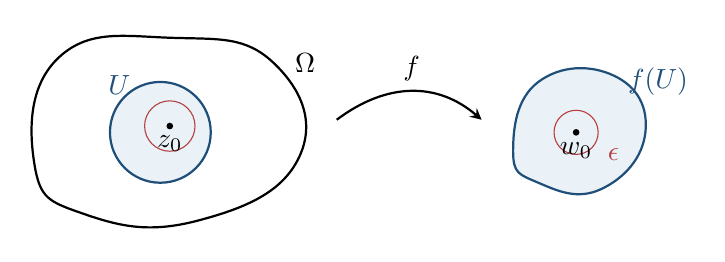
\begin{tikzpicture}[scale=0.8,>=stealth]
 \draw[thick] plot[smooth cycle,tension=0.8] coordinates
 {(-2.6,-0.5) (-2.2,1.2) (-0.4,1.5) (1.2,1.1) (1.6,-0.4) (0,-1.4) (-1.8,-1.3)};
 \node at (1.7,1.1) {$\Omega$};
 \fill[lightblue] (-0.6,0) circle(0.8);
 \draw[courseblue,thick] (-0.6,0) circle(0.8);
 \node[courseblue] at (-1.25,0.75) {$U$};
 \draw[exerciseframe] (-0.45,0.1) circle(0.4);
 \fill (-0.45,0.1) circle(1.5pt) node[below]{$z_0$};
 \draw[->,thick] (2.2,0.2) .. controls (3,0.8) and (3.8,0.8) .. (4.5,0.2)
  node[midway,above]{$f$};
 \begin{scope}[xshift=6cm]
  \fill[lightblue] plot[smooth cycle,tension=0.8] coordinates
   {(-1,-0.3) (-0.6,0.8) (0.6,0.9) (1.1,0) (0.4,-0.9) (-0.6,-0.8)};
  \draw[courseblue,thick] plot[smooth cycle,tension=0.8] coordinates
   {(-1,-0.3) (-0.6,0.8) (0.6,0.9) (1.1,0) (0.4,-0.9) (-0.6,-0.8)};
  \node[courseblue] at (1.3,0.8) {$f(U)$};
  \draw[exerciseframe] (0,0) circle(0.35);
  \fill (0,0) circle(1.5pt) node[below]{$w_0$};
  \node[exerciseframe,right] at (0.35,-0.35) {$\epsilon$};
 \end{scope}
\end{tikzpicture}

{\small Every $w$ within $\epsilon$ of $w_0=f(z_0)$ is attained in the small
disc around $z_0$.}
\end{lecturefigure}

\begin{proof}
The proof follows from Rouch\'e's theorem. Let $w_0\in f(U)$, say
$w_0=f(z_0)$ with $z_0\in U$. We want to show that every $w$ near $w_0$
also lies in the image $f(U)$. Decompose
\[
 f(z)-w=\underbrace{f(z)-w_0}_{F(z)}+\underbrace{w_0-w}_{G(z)}.
\]
The function $F$ has a zero at $z=z_0$. It is not identically zero on
$\Omega$, since $f$ is nonconstant, so by Lemma~\ref{lem:zeros} the zero is
isolated: there is $\delta>0$ with $\overline{D(z_0,\delta)}\subseteq U$ and
$F(z)\ne0$ for $0<|z-z_0|\leq\delta$. On the compact circle
$C_\delta=\{|z-z_0|=\delta\}$, $|F|$ has a positive minimum; pick
$\epsilon>0$ with
\[
 |F(z)|=|f(z)-w_0|>\epsilon\qquad\text{for }z\in C_\delta.
\]
Now if $|w-w_0|<\epsilon$, then $|F(z)|>\epsilon>|w-w_0|=|G(z)|$ for
$z\in C_\delta$. By Rouch\'e's theorem, $F+G=f-w$ has as many zeros in
$D(z_0,\delta)$ as $F$, which has at least one (at $z_0$). So $w=f(z)$ for
some $z\in D(z_0,\delta)\subseteq U$. Thus $D(w_0,\epsilon)\subseteq f(U)$,
and $f(U)$ is open.
\end{proof}

\begin{exercise}[Maximum modulus principle]
Let $f$ be holomorphic and nonconstant on a connected open set $\Omega$.
Use the open mapping theorem to show that $|f|$ has no local maximum in
$\Omega$.
\end{exercise}

\end{document}
